%{
%Formål med afsnit:
%\begin{itemize}
%	\item Problematikken med heltal, herunder hvor tæt vi kommer
%		egentlig på $\varPhi$.
%	\item Hvordan forholder vores approksimation sig ifht. Markovs
%		fejlmargin?
%	\item Vurdering af præcision.
%	\item Fortælle om de hjælpemetoder vi vil få brug for.
%\end{itemize}


\subsection{Hvordan deles billedet efter det gyldne snit}
(intro)

\subsubsection{akseptabel afvigelse}
(her skal der noget ind med at vi egenlide gerne vil have nogle konkrede
tal påm hvor mange $%$ der er aksepeltabel)
I et billedet befinder der sig 4 gyldne snit. 2 i det vertikale plan og
2 i det horisontale plan. placeringen af de 4 snit udregnes i forhold
til udledningen i afsnittet om det gyldne snit, hvor konstanten $\varPhi = 0.618$ 
bliver fundet. Den horisontale brede B og vertikale højte H

\begin{figure}[h]
	\begin{center}
		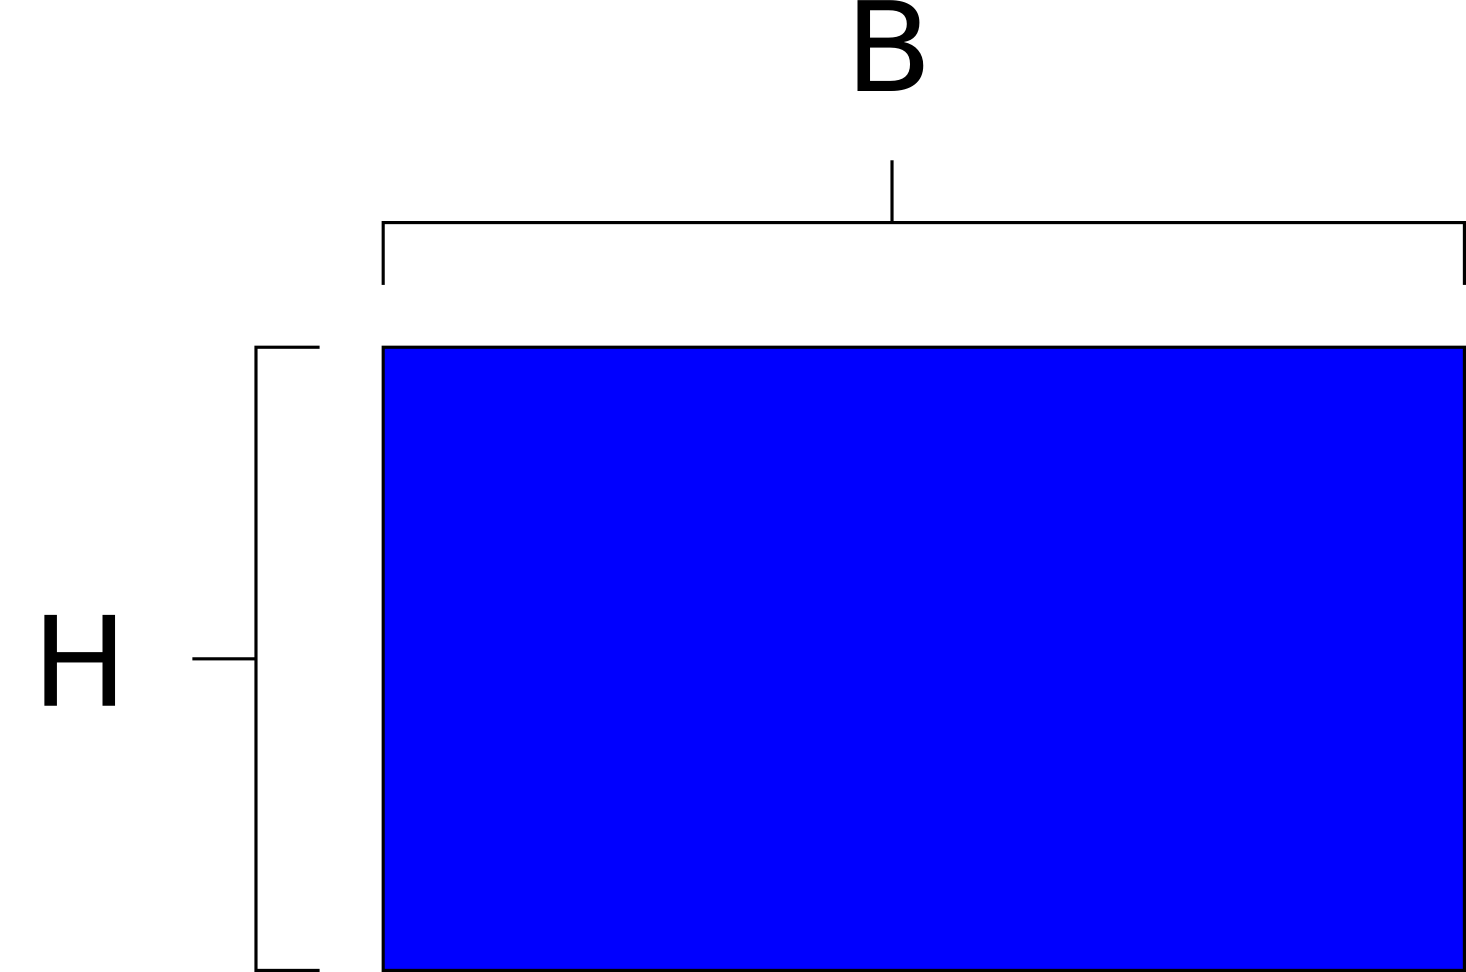
\includegraphics[scale=0.42,angle=0]{afsnit/vores_implementation/billeder/naiv_algoritme/path2407}
	\end{center}
	\caption[]{Billedet opbygning}
	\label{lenasnit}
\end{figure}

bliver divideret med $\varPhi$. Det giver to tal som betegner, hvor
mange pixels fra begge kanter, det gyldne snit befinder sig f.eks ved et
billedet som har B = 4000 pixel, vil punktet ligge ved.

\begin{equation}
	4000/\varPhi = 4000(\sqrt{5}-1)/2 = 2472.13595 \approx 2472
\end{equation}

Som man kan se approsimere vi antal pixel, dette gør at vi har en
usikkerhed på max $0.5$ pixels, dette giver selve i de miste billedet en
$%$ usiker som ligger under 1(dette er godt nok men hvorfor). 

\begin{figure}[h]
	\begin{center}
		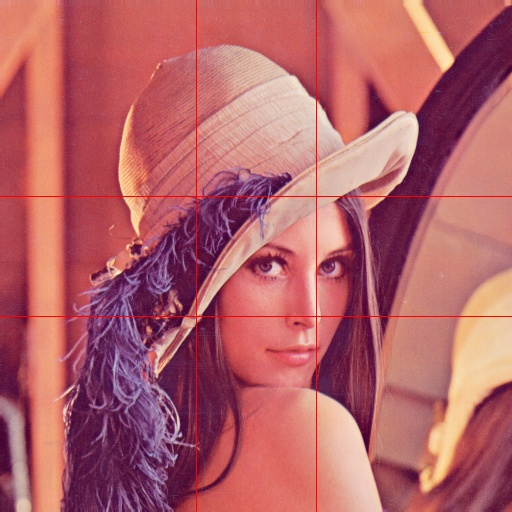
\includegraphics[scale=0.42,angle=0]{afsnit/vores_implementation/billeder/naiv_algoritme/Lenagolden}
	\end{center}
	\caption[]{Billedet som har indtegnet de fire gyldne snit}
	\label{lenasnit2}
\end{figure}

Som man kan se på billedet ser snitne stadig symetriske ud, selv om de
er udregnet ud fra en approsimation.

\subsection*{Problematikken med heltal}
Mange af de metoder som vi bruger til at udregne, position af det gyldne
snit eller størrelsen af en margin, udregnes ved hjælp af brøker.
Tilgængel, er et billedet opbygget af pixels, Dette gør at vi må nød
til at tage approksimationer af udregningerne for at få dem tilbage til et
helt tal, men hvor meget af dataenden er tabt, og hvor maget af
resultaterne kan man stole på.

\subsubsection*{Heltal i det gyldne snit}
Eksemplet med 4000 pixels ovenfor, approksimationen vi antal pixels ved at
runde resultatet, dette gør at vi mister 0.13595 nøjagtighed, dette svare
til en misvisning af punktet på 0.00339875 $\%$ i forholdt til bredden på
billedet. 

\begin{equation}
	0.13595/4000*100 = 0.00339875
\end{equation}

Det er en maget lille del af selve billedet og skulle i give nogle
misvisninger i forhold til udregningen. For at gøre det lidt mere
generat, sætter vi den mistet nøjagtighed til 0.5, det er den Max mistet
nøjagtighed vi kan have, og sætter billedet størrelse til 500(dette er
jeg ikke sikker på,) pixels, som er det miste billedet vi har, dette
giver en fejl margen på 0.1 $\%$. Dette resultat befinder sig stadig
meget lavt, konklutionen er at selv om vi regner med en
approksimation af det gyldne snit få vi stadig et resultat som kan bruges.

\subsubsection{Heltal ved udregning af Margin}
En af vores mål ved denne opgave er at se om kunstnern har tegnet
interessante regioner ved opdelingen af billedet, hvor 2/3 er som snit, og
samme line det med det gyldne snit. Da de 2 snit ligger meget tæt på
hinanden og vi gerne vil lave en sammenligning, er det vigtigt at margin
for snittet ikke krydser hinanden(hvorfor er det vigtigt, og dette en god nok forklaring). Dette vil indebære at de samme
region vil blive fundet af begge snit, og vil give et skævt billedet
af forskellen på de to snit.
hvis x betegner antal pixels i B eller H, og vi vil se
forskellen mellem 2/3 og $\varphi$, multiplisere vi x med snittet for at finde
dens placering og subtrahere dem fra hinanden.

\begin{eqnarray}
	\frac{x3}{2}-\frac{x2}{\sqrt{5}-1} &=& x(\frac{2}{3}-\frac{2}{\sqrt{5}-1}) \\ \nonumber
	&=& x(0.666667-0.618034) \\ \nonumber
	&=& x(0.048633) \\
\end{eqnarray}

Vi har nu fundet antal pixels mellem de to snit. Da vi gerne vil undgå at de to
marginens ikke krydser hinanden, dividere vi med 2 og tager en floor på
helle funktionen.

\begin{equation}
	\lfloor(\frac{\frac{x3}{5} - \frac{x2}{\sqrt{5}+1} }{2})\rfloor
\end{equation}

Dette giver os et antal pixels som skildre de to snit. For at vise
hvor stort marginen egentlige kan være, bruger jeg denne formel på to
billeder, et som svare til vores mindste billedet, 500 pixels, og et
som svare til vores største billedet, 4000 pixels. Ved 500 pixels
bliver resultatet

\begin{equation}
	 \lfloor 500(0.048633)\rfloor = 4
\end{equation}

Det er en ok margin ud fra de udtagelser som vi lavet for to afsnit siden
Ved 4000 pixels giver det.

\begin{equation}
	 \lfloor 4000(0.048633)\rfloor = 36
\end{equation}
(skal lige rengne det igemmen igen  4000(0.048633) ikke = 36)
Som må siges at være mere end nok. nok er nok.
% vim: set tw=72 spell spelllang=da:
